\documentclass[aspectratio=169,11pt]{beamer}

% ================================================================
% "TABIIY TILNI QAYTA ISHLASH" KURSI
% MA'RUZA 7 --- Rekurrent neyron tarmoqlar (RNN)
%              (d07_rnn.tex)
% Arxetiplar: [A][B][C][D][E] + 4 tsikl [F][G][H][I][J][K][L] +
%             [M][N][O][P][Q][R] + ilova [S]
% Rendered slayd soni: ~45 (2-haftaning uchinchi ma'ruzasi; L1-L6 chuqurligi)
% Qulflangan [I2]: h_1 = tanh([1,0]) = [0.762, 0.000]
%   --- P7 (Day 8) birinchi assert manbayi (course_map hand_example).
% ================================================================

% ================================================================
% RANGLAR  (asl fayldan o'zgarishsiz)
% ================================================================
\definecolor{cnublue}{rgb}{0.07,0.14,0.62}
\definecolor{cnubluelight}{rgb}{0.18,0.30,0.72}
\definecolor{cnubluebg}{rgb}{0.90,0.92,0.97}
\definecolor{deepblue}{rgb}{0.07,0.14,0.62}
\definecolor{deepred}{rgb}{0.60,0.00,0.00}
\definecolor{deepgreen}{rgb}{0.00,0.45,0.00}
\definecolor{halfgray}{gray}{0.55}

% ================================================================
% BEAMER MAVZU --- Boadilla + maxsus footer  (asl fayldan o'zgarishsiz)
% ================================================================
\usetheme{Boadilla}

\setbeamercolor{structure}{fg=cnublue}
\setbeamercolor{frametitle}{bg=cnublue,fg=white}
\setbeamercolor{title}{bg=cnublue,fg=white}
\setbeamercolor{block title}{bg=cnublue,fg=white}
\setbeamercolor{block body}{bg=cnubluebg,fg=black}
\setbeamercolor{alerted text}{fg=deepred}
\setbeamercolor{author in head/foot}{bg=cnubluelight,fg=white}
\setbeamercolor{section in head/foot}{bg=cnublue,fg=white}
\setbeamercolor{page number in head/foot}{bg=cnubluelight,fg=white}

\setbeamertemplate{mini frame}{}
\setbeamertemplate{mini frame in current section}{}
\setbeamertemplate{mini frame in current subsection}{}
\setbeamertemplate{headline}{}
\setbeamertemplate{navigation symbols}{}

\setbeamertemplate{footline}{%
  \leavevmode%
  \hbox{%
    \begin{beamercolorbox}[wd=0.17\paperwidth,ht=2.5ex,dp=1.25ex,leftskip=0.5em]{author in head/foot}%
      \usebeamerfont{author in head/foot}\scriptsize\insertshortauthor%
    \end{beamercolorbox}%
    \begin{beamercolorbox}[wd=0.69\paperwidth,ht=2.5ex,dp=1.25ex,center]{section in head/foot}%
      \usebeamerfont{section in head/foot}%
      \scriptsize\insertsectionnavigationhorizontal{0.69\paperwidth}{}{}%
    \end{beamercolorbox}%
    \begin{beamercolorbox}[wd=0.14\paperwidth,ht=2.5ex,dp=1.25ex,rightskip=0.5em]{page number in head/foot}%
      \hfill\scriptsize\color{white}%
      \insertframenumber{}/\inserttotalframenumber%
    \end{beamercolorbox}%
  }%
  \vskip0pt%
}

% ================================================================
% PAKETLAR  (asl fayldan o'zgarishsiz)
% ================================================================
\usepackage[utf8]{inputenc}
\usepackage[T1]{fontenc}
\usepackage{lmodern}
\usepackage{amsmath,amssymb}
\usepackage{booktabs}
\usepackage{xcolor}
\usepackage{listings}
\lstset{
    language=Python,
    basicstyle=\ttfamily\scriptsize,
    keywordstyle=\bfseries\color{deepblue},
    emphstyle=\ttfamily\color{deepred},
    stringstyle=\color{deepgreen},
    commentstyle=\itshape\color{halfgray},
    numbers=left,
    numberstyle=\scriptsize\color{halfgray},
    rulesepcolor=\color{cnublue!30},
    frame=shadowbox,
    breaklines=true,
    showstringspaces=false,
    tabsize=2
}
\usepackage{tcolorbox}
\tcbuselibrary{skins}
\tcbset{
  defbox/.style={colback=cnubluebg,colframe=cnublue,
                 fonttitle=\small\bfseries\color{white},
                 attach boxed title to top left={yshift=-2mm,xshift=4mm},
                 boxed title style={colback=cnublue,colframe=cnublue}},
  warnbox/.style={colback=orange!8,colframe=orange!70!black,
                  fonttitle=\small\bfseries},
  okbox/.style={colback=green!7,colframe=green!55!black,
                fonttitle=\small\bfseries}
}
\usepackage{tikz}
\usetikzlibrary{arrows.meta,positioning}

% ================================================================
% QO'SHIMCHALAR  (asl fayldan o'zgarishsiz)
% ================================================================
\AtBeginSection[]{%
  \begin{frame}{Prezentatsiya rejasi}
    \tableofcontents[currentsection]
  \end{frame}}

\newcommand{\bunda}[1]{{\small\textbf{bunda:}\; #1}}
\newcommand{\bajarildi}{{\color{deepgreen}\large$\checkmark$}\;}

% ================================================================
% METAMA'LUMOT
% ================================================================
\title[RNN]{Rekurrent neyron tarmoqlar (RNN)}
\subtitle{Tabiiy tilni qayta ishlash --- 7-ma'ruza}
\author[A.A.\,Abdulali]{A.A.\,Abdulali}
\date{25-iyun 2026}
\institute{11:00--12:20 \quad$\cdot$\quad mavzu \textnumero{}7}

% ================================================================
\begin{document}
% ================================================================

% ----------------------------------------------------------------
% [A] TITUL
% ----------------------------------------------------------------
\maketitle

% ================================================================
\section[Kirish]{Kirish: ketma-ketlikni xotira bilan modellaymiz}
% ================================================================

% ----------------------------------------------------------------
% [B] TAKRORLASH: L5+L6 va bugungi P6
% ----------------------------------------------------------------
\begin{frame}{Takrorlash: o'tgan darslardan ikki savol}
  \begin{columns}[T]
    \begin{column}{0.49\textwidth}
      \begin{tcolorbox}[warnbox,title=1-savol]
        \small
        L5 da bigram faqat \textbf{1 oldingi} so'zga qaradi. ``men kitobni
        do'stimga \underline{\hspace{0.7cm}}'' --- kesim uzoqda. Sobit oyna uzoq
        bog'liqlikni ko'ra oladimi?
      \end{tcolorbox}
    \end{column}
    \begin{column}{0.49\textwidth}
      \begin{tcolorbox}[warnbox,title=2-savol]
        \small
        Bugun ertalab P6 da Word2Vec har \textbf{so'zga} vektor berdi. Lekin gap
        --- so'zlar \textbf{ketma-ketligi}. Embedding o'zi tartibni/xotirani
        saqlaydimi?
      \end{tcolorbox}
    \end{column}
  \end{columns}
  \pause
  \vspace{4pt}
  \begin{columns}[T]
    \begin{column}{0.49\textwidth}
      \begin{tcolorbox}[okbox,title=1-javob]
        \small
        \textbf{Yo'q.} Sobit oyna faqat $n{-}1$ so'zni ko'radi; undan uzoqdagi
        kesim ko'rinmaydi (Markov cheklovi).
      \end{tcolorbox}
    \end{column}
    \begin{column}{0.49\textwidth}
      \begin{tcolorbox}[okbox,title=2-javob]
        \small
        \textbf{Yo'q.} Har vektor mustaqil --- ketma-ketlik tartibi yo'qoladi.
        Bugun \textbf{xotirali} model quramiz: RNN.
      \end{tcolorbox}
    \end{column}
  \end{columns}
\end{frame}

% ----------------------------------------------------------------
% [C] MAQSADLAR
% ----------------------------------------------------------------
\begin{frame}{Siz bugungi dars oxirida quyidagilarni bajara olasiz:}
  \begin{enumerate}\setlength\itemsep{6pt}
    \item \textbf{Tushuntira olasiz:} nega sobit oyna (N-gram/feedforward) uzoq
          bog'liqlikni ushlay olmaydi.
    \item \textbf{Hisoblay olasiz:} RNN bir qadamini qo'lda ---
          $h_t=\tanh(W_h h_{t-1}+W_x x_t)$, $h_1=[0.762,0.000]$.
    \item \textbf{Tushuntira olasiz:} vaqt bo'ylab yoyilish (unrolling), og'irliklar
          ulashilishi va BPTT g'oyasini.
    \item \textbf{Qo'llay olasiz:} RNN ni til modellashtirish va matn tasniflashda
          (ko'p-dan-bir).
  \end{enumerate}
  \vspace{4pt}
  \begin{tcolorbox}[defbox,title=Oldindan talab]
    \footnotesize
    L5 dan: til modeli, Markov taxmini. L6 dan: embedding (kirish vektori), softmax,
    gradient. Matematikadan: matritsa-vektor ko'paytma, $\tanh$, zanjir qoidasi.
  \end{tcolorbox}
\end{frame}

% ----------------------------------------------------------------
% [D] REJA
% ----------------------------------------------------------------
\begin{frame}{Bugungi dars rejasi:}
  \begin{center}
  \small
  \begin{tabular}{c p{5.2cm} c p{3.0cm}}
    \toprule
    \textbf{Tsikl}& \textbf{Mavzu} & \textbf{Vaqt} & \textbf{Hosil bo'luvchi natija}\\
    \midrule
    1 & Sobit oynadan ketma-ket xotiraga & 16 daq & Oyna cheklovi \\
    2 & RNN konsepsiyasi: yashirin holat & 20 daq & $h_1=[0.762,0.000]$ \\
    3 & Vaqt bo'ylab yoyilish va BPTT & 18 daq & $h_2=[0.642,0.762]$ \\
    4 & Til modeli va matn tasniflash & 16 daq & softmax $\to$ ijobiy \\
    \midrule
      & Xulosa va 7-amaliyotga ko'rsatmalar & 10 daq & Ertaga nima qurishingiz \\
    \bottomrule
  \end{tabular}
  \end{center}
  \vspace{4pt}
  \begin{tcolorbox}[warnbox,title=Bu dars neyron ketma-ketlik modellarini ochadi]
    \footnotesize\sloppy
    N-gram (L5) va embedding (L6) dan \textbf{rekurrent} modellarga o'tamiz.
    Bugungi $h_1=[0.762,0.000]$ ertangi P7 da \texttt{assert} bo'ladi.
  \end{tcolorbox}
\end{frame}

% ----------------------------------------------------------------
% [E] MUAMMO BIRINCHI
% ----------------------------------------------------------------
\begin{frame}{Bugungi dars uchun muammo: gap uzunligi har xil, kesim uzoqda}
  \begin{columns}[T]
    \begin{column}{0.50\textwidth}
      \textbf{Sodda yechim qayerda qiynaladi:}\\[3pt]
      \small
      \begin{tcolorbox}[warnbox,title={Sobit oyna ko'r},top=2pt,bottom=2pt]
        \footnotesize
        Embeddinglarni \textbf{sobit} oynada birlashtiramiz (feedforward LM).
        \texttt{"men kitobni do'stimga berdim"} --- kesim \texttt{berdim} oynadan
        tashqarida qolsa, ko'rinmaydi.
      \end{tcolorbox}
      \vspace{3pt}
      \begin{tcolorbox}[warnbox,title={Oynani kattalashtirish qimmat},top=2pt,bottom=2pt]
        \footnotesize
        Oyna $k$ ortsa, parametrlar soni ham ortadi; baribir \textbf{chegaralangan}
        uzunlik.
      \end{tcolorbox}
    \end{column}
    \begin{column}{0.46\textwidth}
      \textbf{Bugungi yechim:}\\[4pt]
      \small
      \begin{enumerate}\setlength\itemsep{4pt}
        \item So'zlarni \textbf{birma-bir} o'qiymiz.
        \item Har qadamda \textbf{yashirin holat}ni (xotira) yangilaymiz.
        \item Holat o'tmishning ``xulosasi'' --- ixtiyoriy uzunlikni ushlaydi.
      \end{enumerate}
      \vspace{5pt}
      \begin{tcolorbox}[okbox,top=2pt,bottom=2pt]
        \footnotesize
        Bu g'oyaning nomi --- \textbf{rekurrent neyron tarmoq (RNN)}: bir xil
        amalni ketma-ketlik bo'ylab \textbf{takrorlaydi}.
      \end{tcolorbox}
    \end{column}
  \end{columns}
\end{frame}

% ================================================================
\section[Neyron LM]{Sobit oynadan ketma-ket xotiraga}
% ================================================================

% ----------------------------------------------------------------
% [F1] INTUITSIYA
% ----------------------------------------------------------------
\begin{frame}{Intuitsiya: sobit oyna --- ``teshikdan'' qarash}
  \begin{columns}[T]
    \begin{column}{0.52\textwidth}
      \small
      Feedforward neyron til modeli: oxirgi $k$ so'z embeddingini
      \textbf{birlashtirib} (concat) keyingisini bashorat qiladi.\\[6pt]
      \texttt{[men][kitobni]} $\to$ keyingi so'z?\\[6pt]
      Muammo: $k$ \textbf{sobit}. $k$ dan uzoqdagi so'z umuman kirmaydi ---
      xuddi tor teshikdan qaragandek.
    \end{column}
    \begin{column}{0.44\textwidth}
      \begin{tcolorbox}[okbox,top=2pt,bottom=2pt]
        \footnotesize
        N-gram sanadi, feedforward LM \textbf{o'rganadi} --- lekin ikkalasi ham
        sobit oynaga bog'liq. Bizga oyna emas, \textbf{xotira} kerak.
      \end{tcolorbox}
    \end{column}
  \end{columns}
\end{frame}

% ----------------------------------------------------------------
% [G1] RASMIY TA'RIF + BUNDA
% ----------------------------------------------------------------
\begin{frame}{Feedforward neyron til modeli: rasmiy ta'rif}
  \begin{tcolorbox}[defbox,title=Ta'rif: sobit-oynali neyron LM]
    \vspace{-0.4em}
    $$ \mathbf{c} = [\mathbf{e}_{w_{t-k}};\ \ldots;\ \mathbf{e}_{w_{t-1}}], \qquad
       \hat{\mathbf{y}} = \mathrm{softmax}(W\,\mathbf{c}+\mathbf{b}) $$
  \end{tcolorbox}
  \vspace{3pt}
  \bunda{$\mathbf{e}_{w}$ --- $w$ so'zning embeddingi (L6); $[\,;\,]$ ---
  \textbf{birlashtirish} (concatenation); $k$ --- sobit oyna o'lchami;
  $\mathbf{c}$ --- $k\cdot d$ o'lchamli kirish; $\hat{\mathbf{y}}$ --- lug'at
  ustidan keyingi so'z taqsimoti.}
  \vspace{5pt}
  \textbf{Diqqat:} kirish o'lchami $k\cdot d$ --- \textbf{sobit}. Gap uzunligi
  o'zgaruvchan bo'lsa ham, model faqat $k$ ta so'zni ko'radi.
\end{frame}

% ----------------------------------------------------------------
% [H1] KELTIRIB CHIQARISH
% ----------------------------------------------------------------
\begin{frame}{Keltirib chiqarish: nega sobit oyna uzoq bog'liqlikni uzadi?}
  \textbf{1-qadam.} Bashorat faqat $\mathbf{c}=[\mathbf{e}_{w_{t-k}};\ldots;\mathbf{e}_{w_{t-1}}]$
  ga bog'liq --- $k$ so'zdan narisi kirmaydi.
  \pause
  \textbf{2-qadam.} O'zbekcha SOV: \textit{``men kitobni do'stimga berdim''} ---
  kesim \texttt{berdim} gap oxirida. Agar $k=2$ bo'lsa, \texttt{men}/\texttt{kitobni}
  \texttt{berdim} ni bashoratlashga ta'sir qila olmaydi.
  \pause
  \textbf{3-qadam.} $k$ ni oshirish --- $W$ o'lchami $k\cdot d$ ga proporsional ortadi
  (parametr portlashi), va baribir uzunlik \textbf{chegaralangan}.
  \begin{tcolorbox}[okbox,top=2pt,bottom=2pt]
    \small \textbf{Xulosa:} kerakli narsa --- sobit oyna emas, o'tmishni
    \textbf{ixcham holat}ga jamlaydigan mexanizm. Bu --- RNN.
  \end{tcolorbox}
\end{frame}

% ----------------------------------------------------------------
% [I1] QO'LDA MISOL
% ----------------------------------------------------------------
\begin{frame}{Qo'lda misol: kontekst vektorini birlashtirish}
  \begin{tcolorbox}[defbox,title={Oyna k=2, embedding o'lchami d=2}]
    \small
    $\mathbf{e}_{\text{men}}=[0.5,0.3]$, \quad $\mathbf{e}_{\text{kitobni}}=[0.2,0.6]$.
  \end{tcolorbox}
  \vspace{0.2em}
  \begin{columns}[T]
    \begin{column}{0.52\textwidth}
      \textbf{Birlashtiramiz:}
      \begin{align*}
        \mathbf{c} &= [\mathbf{e}_{\text{men}};\ \mathbf{e}_{\text{kitobni}}]\\
          &= [0.5,\,0.3,\,0.2,\,0.6]
      \end{align*}
      Kirish o'lchami $= k\cdot d = 2\cdot 2 = 4$.
    \end{column}
    \begin{column}{0.44\textwidth}
      \begin{tcolorbox}[okbox,top=2pt,bottom=2pt]
        \footnotesize
        Uchinchi so'z qo'shilsa, $\mathbf{c}$ \textbf{6} o'lchamli bo'lardi ---
        $W$ ham kattalashadi. Sobit $k$ shuning uchun zarur, ammo cheklovchi.
      \end{tcolorbox}
    \end{column}
  \end{columns}
\end{frame}

% ----------------------------------------------------------------
% [J1] SIZNING VAZIFANGIZ
% ----------------------------------------------------------------
\begin{frame}{Sizning vazifangiz: yana bir birlashtirish}
  \begin{tcolorbox}[warnbox,title=Savol --- 60 soniya]
    \small
    $\mathbf{e}_{\text{u}}=[0.1,0.9]$, \quad $\mathbf{e}_{\text{keldi}}=[0.4,0.4]$,
    oyna $k=2$:\\[4pt]
    \textbf{\large $\mathbf{c} = ?$ \quad va uning o'lchami nechta?}
  \end{tcolorbox}
  \pause
  \begin{tcolorbox}[okbox,title=Javob]
    \small
    $\mathbf{c} = [\mathbf{e}_{\text{u}};\ \mathbf{e}_{\text{keldi}}]
       = [0.1,\,0.9,\,0.4,\,0.4]$, \quad o'lcham $= 2\cdot 2 = \mathbf{4}$.\\[3pt]
    \footnotesize Har qo'shilgan so'z kirishni $d$ ga kattalashtiradi --- model
    o'zgaruvchan uzunlikka moslasha olmaydi.
  \end{tcolorbox}
\end{frame}

% ----------------------------------------------------------------
% [K1] KOD <-> FORMULA  [fragile]
% ----------------------------------------------------------------
\begin{frame}[fragile]{Kod $\leftrightarrow$ formula: sobit-oynali kirish}
  \begin{columns}[T]
    \begin{column}{0.56\textwidth}
\begin{lstlisting}
import numpy as np

e_men     = np.array([0.5, 0.3])
e_kitobni = np.array([0.2, 0.6])

# sobit oyna: embeddinglarni birlashtirish
c = np.concatenate([e_men, e_kitobni])
print(c, c.shape)   # [0.5 0.3 0.2 0.6] (4,)

# W ning ustun soni = k * d ga bog'liq (sobit)
W = np.random.randn(10, c.shape[0])
\end{lstlisting}
    \end{column}
    \begin{column}{0.40\textwidth}
      \textbf{Kod $\to$ formula:}\\[3pt]
      \footnotesize
      \begin{tabular}{p{2.0cm}p{2.0cm}}
        \toprule
        Kod & Formula \\
        \midrule
        \texttt{concatenate} & $[\mathbf{e};\mathbf{e}]$ \\
        \texttt{c.shape} & $k\cdot d$ \\
        \texttt{W @ c} & $W\mathbf{c}$ \\
        \bottomrule
      \end{tabular}
      \vspace{4pt}
      \begin{tcolorbox}[warnbox,top=2pt,bottom=2pt]
        \footnotesize
        \texttt{W} ning kengligi sobit --- gap uzunligiga moslasha olmaydi.
        RNN buni hal qiladi.
      \end{tcolorbox}
    \end{column}
  \end{columns}
\end{frame}

% ----------------------------------------------------------------
% [L1] TUZOG'
% ----------------------------------------------------------------
\begin{frame}{Sobit oyna tuzog'i: ikki yomon tanlov}
  \begin{columns}[T]
    \begin{column}{0.52\textwidth}
      \begin{tcolorbox}[warnbox,title=Murosa]
        \small
        \begin{itemize}\setlength\itemsep{2pt}
          \item Kichik $k$ $\Rightarrow$ uzoq bog'liqlik yo'qoladi.
          \item Katta $k$ $\Rightarrow$ parametr portlashi, ortiqcha moslashish.
          \item Har holatda uzunlik \textbf{chegaralangan}.
        \end{itemize}
      \end{tcolorbox}
    \end{column}
    \begin{column}{0.44\textwidth}
      \begin{tcolorbox}[okbox,top=2pt,bottom=2pt]
        \footnotesize
        \textbf{Yechim:} o'tmishni sobit o'lchamli \textbf{holat}ga jamlash va
        uni har qadamda \textbf{bir xil} og'irliklar bilan yangilash --- RNN
        (2-tsikl).
      \end{tcolorbox}
    \end{column}
  \end{columns}
\end{frame}

% ================================================================
\section[RNN]{RNN konsepsiyasi: yashirin holat}
% ================================================================

% ----------------------------------------------------------------
% [F2] INTUITSIYA
% ----------------------------------------------------------------
\begin{frame}{Intuitsiya: o'qiyotganda ``xayolda'' xulosa saqlaymiz}
  \begin{columns}[T]
    \begin{column}{0.52\textwidth}
      \small
      Gapni o'qiyotganda har so'zdan keyin \textbf{tushunchamizni} yangilaymiz ---
      boshidan qayta o'qimaymiz.\\[6pt]
      RNN ham shunday: \textbf{yashirin holat} $h_t$ --- ``shu paytgacha
      o'qilganlarning xulosasi''.\\[4pt]
      Har qadam: $h_t$ --- oldingi holat $h_{t-1}$ va joriy so'z $x_t$ dan.
    \end{column}
    \begin{column}{0.44\textwidth}
      \begin{tcolorbox}[okbox,top=2pt,bottom=2pt]
        \footnotesize
        Bir xil amal (bir xil $W_h, W_x$) har qadamda \textbf{takrorlanadi} ---
        shuning uchun ``rekurrent''. Uzunlik muhim emas.
      \end{tcolorbox}
    \end{column}
  \end{columns}
\end{frame}

% ----------------------------------------------------------------
% [G2] RASMIY TA'RIF + BUNDA
% ----------------------------------------------------------------
\begin{frame}{RNN rekurrensiyasi: rasmiy ta'rif}
  \begin{tcolorbox}[defbox,title=Ta'rif: RNN yashirin holati]
    \vspace{-0.4em}
    $$ h_t = \tanh\!\big(W_h\,h_{t-1} + W_x\,x_t + b\big) $$
  \end{tcolorbox}
  \vspace{3pt}
  \bunda{$x_t$ --- $t$ qadamdagi kirish (so'z embeddingi); $h_t$ --- yashirin holat
  (xotira); $W_h$ --- holat$\to$holat, $W_x$ --- kirish$\to$holat og'irliklari;
  $b$ --- bias; $\tanh$ --- nochiziqlilik; $h_0=\mathbf{0}$.}
  \vspace{4pt}
  \textbf{Asosiy nuqta:} $W_h, W_x$ \textbf{barcha qadamlarda bir xil} (ulashilgan).
  Holat o'lchami sobit --- gap uzunligidan mustaqil.
\end{frame}

% ----------------------------------------------------------------
% [H2] KELTIRIB CHIQARISH
% ----------------------------------------------------------------
\begin{frame}{Keltirib chiqarish: rekurrensiya qayerdan keladi?}
  \textbf{1-qadam.} Maqsad: butun o'tmish $x_1\ldots x_t$ ni \textbf{sobit
  o'lchamli} holatga jamlash.
  \pause
  \textbf{2-qadam.} Rekursiv ta'rif --- yangi holat eski holat va yangi kirishdan:
  $$ h_t = f(h_{t-1},\, x_t) $$
  \pause
  \textbf{3-qadam.} $f$ ni eng sodda o'rganiladigan ko'rinishda olamiz: chiziqli
  birikma $+$ nochiziqlilik:
  $$ h_t = \tanh(W_h h_{t-1} + W_x x_t + b) $$
  \begin{tcolorbox}[okbox,top=2pt,bottom=2pt]
    \small \textbf{Xulosa:} $h_t$ rekursiya orqali $x_1\ldots x_t$ ning hammasiga
    bog'liq --- sobit oyna yo'q. $\tanh$ holatni $[-1,1]$ da ushlaydi.
  \end{tcolorbox}
\end{frame}

% ----------------------------------------------------------------
% [I2] QO'LDA MISOL --- QULFLANGAN TRACEABILITY SLAYD
%
% P7 (Day 8) birinchi assert bilan solishtiring:
%   h_1 = tanh([1,0]) = [0.762, 0.000]   [Ma'ruza L7 [I2]-slayd]
% course_map.yaml hand_example verbatim.
% ----------------------------------------------------------------
\begin{frame}{Qo'lda misol: RNN bir qadami --- $h_1=[0.762,\,0.000]$}
  \begin{tcolorbox}[defbox,title={$h_0=[0,0]$;\ $W_h=I$,\ $W_x=I$;\ $x_1=[1,0]$}]
    \small
    $W_h=W_x=\left(\begin{smallmatrix}1&0\\0&1\end{smallmatrix}\right)$ (birlik matritsa),
    \; $b=\mathbf{0}$, \; $h_0=[0,0]$.
  \end{tcolorbox}
  \vspace{0.2em}
  \begin{columns}[T]
    \begin{column}{0.54\textwidth}
      \textbf{Hisoblaymiz:}
      \begin{align*}
        h_1 &= \tanh(W_h h_0 + W_x x_1)\\
            &= \tanh([0,0] + [1,0])\\
            &= [\tanh(1),\ \tanh(0)]\\
            &= \mathbf{[0.762,\ 0.000]}
      \end{align*}
    \end{column}
    \begin{column}{0.42\textwidth}
      \begin{tcolorbox}[okbox,top=2pt,bottom=2pt]
        \footnotesize
        $\tanh(1)\approx 0.7616$, $\tanh(0)=0$. Holat birinchi so'zning
        ``izi''ni saqladi.
      \end{tcolorbox}
      \vspace{3pt}
      \footnotesize\color{halfgray}
      Ertangi P7 birinchi assert:\\
      \texttt{np.allclose(h1,}\\
      \texttt{\phantom{xx}[0.762, 0.0], atol=1e-3)}\\
      \textit{\# Ma'ruza L7 [I2]-slayd}
    \end{column}
  \end{columns}
\end{frame}

% ----------------------------------------------------------------
% [J2] SIZNING VAZIFANGIZ
% ----------------------------------------------------------------
\begin{frame}{Sizning vazifangiz: boshqa kirish uchun $h_1$}
  \begin{tcolorbox}[warnbox,title=Savol --- 90 soniya]
    \small
    Xuddi shu RNN ($W_h=W_x=I$, $b=0$, $h_0=[0,0]$), lekin $x_1=[0,1]$:\\[4pt]
    \textbf{\large $h_1 = ?$}
  \end{tcolorbox}
  \pause
  \begin{tcolorbox}[okbox,title=Javob]
    \small
    $h_1 = \tanh([0,0]+[0,1]) = [\tanh(0),\ \tanh(1)] = \mathbf{[0.000,\ 0.762]}$\\[3pt]
    \footnotesize Kirish ikkinchi o'lchamda edi $\Rightarrow$ ``iz'' ham ikkinchi
    o'lchamda. Birlik matritsada har kirish o'z o'rnida saqlanadi.
  \end{tcolorbox}
\end{frame}

% ----------------------------------------------------------------
% [K2] KOD <-> FORMULA  [fragile]
% ----------------------------------------------------------------
\begin{frame}[fragile]{Kod $\leftrightarrow$ formula: RNN bir qadami}
  \begin{columns}[T]
    \begin{column}{0.56\textwidth}
\begin{lstlisting}
import numpy as np

Wh = np.eye(2)        # I_2
Wx = np.eye(2)        # I_2
b  = np.zeros(2)

def rnn_step(h_prev, x):
    return np.tanh(Wh @ h_prev + Wx @ x + b)

h0 = np.zeros(2)
h1 = rnn_step(h0, np.array([1.0, 0.0]))
print(h1)             # [0.762 0.0]
\end{lstlisting}
    \end{column}
    \begin{column}{0.40\textwidth}
      \textbf{Kod $\to$ formula:}\\[3pt]
      \footnotesize
      \begin{tabular}{p{2.0cm}p{2.0cm}}
        \toprule
        Kod & Formula \\
        \midrule
        \texttt{Wh @ h\_prev} & $W_h h_{t-1}$ \\
        \texttt{Wx @ x} & $W_x x_t$ \\
        \texttt{np.tanh(...)} & $\tanh(\cdot)$ \\
        \bottomrule
      \end{tabular}
      \vspace{4pt}
      \begin{tcolorbox}[okbox,top=2pt,bottom=2pt]
        \footnotesize
        Ertangi P7 da \texttt{m07 RNNClassifier} aynan shu qadamni (PyTorch
        \texttt{nn.RNN}) ishlatadi.
      \end{tcolorbox}
    \end{column}
  \end{columns}
\end{frame}

% ----------------------------------------------------------------
% [L2] TUZOG'
% ----------------------------------------------------------------
\begin{frame}{RNN tuzog'i: holatni boshlash va tartib muhim}
  \begin{columns}[T]
    \begin{column}{0.52\textwidth}
      \begin{tcolorbox}[warnbox,title=Keng tarqalgan xatolar]
        \small
        \begin{itemize}\setlength\itemsep{2pt}
          \item $h_0$ ni unutib, oldingi gap holatini olib qolish.
          \item So'z tartibini buzish --- RNN tartibga \textbf{sezgir}
                (``it odamni qopdi'' $\neq$ ``odam itni qopdi'').
          \item $\tanh$ o'rniga noto'g'ri nochiziqlilik.
        \end{itemize}
      \end{tcolorbox}
    \end{column}
    \begin{column}{0.44\textwidth}
      \begin{tcolorbox}[okbox,top=2pt,bottom=2pt]
        \footnotesize
        \textbf{Yechim:} har ketma-ketlik uchun $h_0=\mathbf{0}$ dan boshlang;
        so'z tartibini saqlang. Tartibga sezgirlik --- RNN ning \textbf{kuchi}.
      \end{tcolorbox}
    \end{column}
  \end{columns}
\end{frame}

% ================================================================
\section[Yoyilish]{Vaqt bo'ylab yoyilish va BPTT}
% ================================================================

% ----------------------------------------------------------------
% [F3] INTUITSIYA + TikZ
% ----------------------------------------------------------------
\begin{frame}{Intuitsiya: bir katakni vaqt bo'ylab yoyamiz}
  \begin{center}
  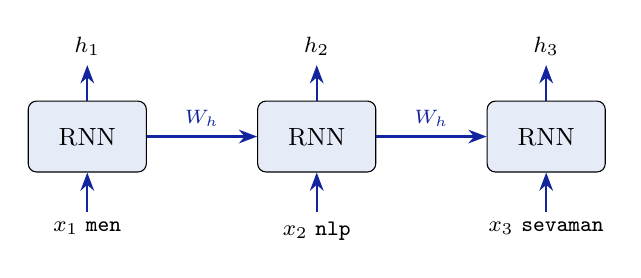
\begin{tikzpicture}[
      cell/.style={draw, fill=cnubluebg, rounded corners=3pt,
                   minimum width=1.5cm, minimum height=0.9cm, font=\small, align=center},
      io/.style={font=\footnotesize},
      arr/.style={-{Stealth}, thick, color=cnublue}
  ]
    \node[cell] (h1) {RNN};
    \node[cell, right=1.4cm of h1] (h2) {RNN};
    \node[cell, right=1.4cm of h2] (h3) {RNN};
    \node[io, below=0.5cm of h1] (x1) {$x_1$ \texttt{men}};
    \node[io, below=0.5cm of h2] (x2) {$x_2$ \texttt{nlp}};
    \node[io, below=0.5cm of h3] (x3) {$x_3$ \texttt{sevaman}};
    \node[io, above=0.45cm of h1] (o1) {$h_1$};
    \node[io, above=0.45cm of h2] (o2) {$h_2$};
    \node[io, above=0.45cm of h3] (o3) {$h_3$};
    \draw[arr] (x1)--(h1); \draw[arr] (x2)--(h2); \draw[arr] (x3)--(h3);
    \draw[arr] (h1)--(o1); \draw[arr] (h2)--(o2); \draw[arr] (h3)--(o3);
    \draw[arr] (h1)--(h2) node[midway,above,font=\scriptsize]{$W_h$};
    \draw[arr] (h2)--(h3) node[midway,above,font=\scriptsize]{$W_h$};
  \end{tikzpicture}
  \end{center}
  \vspace{4pt}
  \begin{tcolorbox}[okbox,top=2pt,bottom=2pt]
    \footnotesize
    Bu --- \textbf{bitta} katakning uch qadamga ``yoyilgani'' (unrolling). Uchala
    nusxa \textbf{bir xil} $W_h, W_x$ ni ulashadi --- shuning uchun har xil uzunlikdagi
    gaplar uchun ishlaydi.
  \end{tcolorbox}
\end{frame}

% ----------------------------------------------------------------
% [G3] RASMIY TA'RIF + BUNDA
% ----------------------------------------------------------------
\begin{frame}{Yoyilish va BPTT: rasmiy ta'rif}
  \begin{tcolorbox}[defbox,title=Ta'rif: vaqt bo'ylab teskari tarqalish (BPTT)]
    \vspace{-0.4em}
    $$ \frac{\partial \mathcal{L}}{\partial W_h}
       = \sum_{t=1}^{T} \frac{\partial \mathcal{L}_t}{\partial W_h},
       \qquad
       \frac{\partial h_t}{\partial h_{t-1}} = \mathrm{diag}\!\big(1-h_t^2\big)\,W_h $$
  \end{tcolorbox}
  \vspace{2pt}
  \bunda{$T$ --- ketma-ketlik uzunligi; yoyilgan tarmoq oddiy chuqur tarmoqdek;
  $W_h$ \textbf{ulashilgani} uchun gradientlar barcha qadamlar bo'ylab
  \textbf{yig'iladi}; $1-h_t^2$ --- $\tanh$ hosilasi.}
  \vspace{4pt}
  \footnotesize Yoyilgandan keyin --- bu shunchaki chuqur tarmoq; oddiy backprop
  qo'llanadi, faqat $W_h$ takror ishlatilgani uchun gradientlar qo'shiladi.
\end{frame}

% ----------------------------------------------------------------
% [H3] KELTIRIB CHIQARISH
% ----------------------------------------------------------------
\begin{frame}{Keltirib chiqarish: gradient nega qadamlar ko'paytmasi?}
  \textbf{1-qadam.} $h_T$ uzoq $h_{t}$ ga zanjir qoidasi orqali bog'liq:
  $$ \frac{\partial h_T}{\partial h_t} = \prod_{s=t+1}^{T} \frac{\partial h_s}{\partial h_{s-1}} $$
  \pause
  \textbf{2-qadam.} Har bo'g'in $\dfrac{\partial h_s}{\partial h_{s-1}}
  = \mathrm{diag}(1-h_s^2)\,W_h$ --- \textbf{ko'paytma} hosil bo'ladi.
  \pause
  \textbf{3-qadam.} Ko'p bo'g'in ko'paytmasi: agar har bo'g'in $<1$ bo'lsa, ko'paytma
  \textbf{eksponensial so'nadi} (vanishing); $>1$ bo'lsa portlaydi (exploding).
  \begin{tcolorbox}[okbox,top=2pt,bottom=2pt]
    \small \textbf{Xulosa:} uzoq bog'liqlik gradienti so'nadi $\Rightarrow$ RNN
    uzoq xotirani \textbf{o'rganishda qiynaladi}. Bu --- L8 (LSTM/GRU) sababi.
  \end{tcolorbox}
\end{frame}

% ----------------------------------------------------------------
% [I3] QO'LDA MISOL
% ----------------------------------------------------------------
\begin{frame}{Qo'lda misol: ikkinchi qadam --- $h_2=[0.642,\,0.762]$}
  \begin{tcolorbox}[defbox,title={Davomi: $h_1=[0.762,0]$,\ $x_2=[0,1]$,\ $W_h=W_x=I$}]
    \small $h_1=[0.762,\,0.000]$ (oldingi tsikldan), \; $x_2=[0,1]$.
  \end{tcolorbox}
  \vspace{0.2em}
  \begin{columns}[T]
    \begin{column}{0.54\textwidth}
      \textbf{Hisoblaymiz:}
      \begin{align*}
        h_2 &= \tanh(W_h h_1 + W_x x_2)\\
            &= \tanh([0.762,0] + [0,1])\\
            &= [\tanh(0.762),\ \tanh(1)]\\
            &= \mathbf{[0.642,\ 0.762]}
      \end{align*}
    \end{column}
    \begin{column}{0.42\textwidth}
      \begin{tcolorbox}[okbox,top=2pt,bottom=2pt]
        \footnotesize
        $\tanh(0.762)\approx 0.642$. Holat endi \textbf{ikkala} so'zning izini
        saqlaydi --- xotira ketma-ket to'planadi.
      \end{tcolorbox}
    \end{column}
  \end{columns}
\end{frame}

% ----------------------------------------------------------------
% [J3] SIZNING VAZIFANGIZ
% ----------------------------------------------------------------
\begin{frame}{Sizning vazifangiz: $\tanh$ hosilasini bahola}
  \begin{tcolorbox}[warnbox,title=Savol --- 90 soniya]
    \small
    BPTT bo'g'inida $\tanh$ hosilasi $1-h^2$. Agar holat komponenti $h=0.762$
    bo'lsa:\\[4pt]
    \textbf{\large $1-h^2 = ?$ \quad (bu $<1$ mi?)}
  \end{tcolorbox}
  \pause
  \begin{tcolorbox}[okbox,title=Javob]
    \small
    $1 - 0.762^2 = 1 - 0.581 = \mathbf{0.419}$ \; ($<1$).\\[3pt]
    \footnotesize Har bo'g'in $\approx 0.42$ bo'lsa, 10 qadamdan keyin
    $0.42^{10}\approx 1.7\times10^{-4}$ --- gradient \textbf{so'nadi}. Mana
    vanishing gradient.
  \end{tcolorbox}
\end{frame}

% ----------------------------------------------------------------
% [K3] KOD <-> FORMULA  [fragile]
% ----------------------------------------------------------------
\begin{frame}[fragile]{Kod $\leftrightarrow$ formula: ketma-ketlik bo'ylab aylanish}
  \begin{columns}[T]
    \begin{column}{0.56\textwidth}
\begin{lstlisting}
import numpy as np

Wh = np.eye(2); Wx = np.eye(2)

def rnn_forward(xs, h0):
    h = h0
    for x in xs:                 # vaqt bo'ylab yoyilish
        h = np.tanh(Wh @ h + Wx @ x)
    return h

xs = [np.array([1.0, 0.0]),
      np.array([0.0, 1.0])]
hT = rnn_forward(xs, np.zeros(2))
print(hT)                        # [0.642 0.762]
\end{lstlisting}
    \end{column}
    \begin{column}{0.40\textwidth}
      \textbf{Kod $\to$ formula:}\\[3pt]
      \footnotesize
      \begin{tabular}{p{2.0cm}p{2.0cm}}
        \toprule
        Kod & Formula \\
        \midrule
        \texttt{for x in xs} & $t=1\ldots T$ \\
        \texttt{h = tanh(...)} & $h_t$ rekursiya \\
        \texttt{return h} & $h_T$ \\
        \bottomrule
      \end{tabular}
      \vspace{4pt}
      \begin{tcolorbox}[okbox,top=2pt,bottom=2pt]
        \footnotesize
        Bir xil \texttt{Wh, Wx} har aylanishda --- og'irliklar ulashilishi.
        Sikl --- yoyilishning kod ko'rinishi.
      \end{tcolorbox}
    \end{column}
  \end{columns}
\end{frame}

% ----------------------------------------------------------------
% [L3] TUZOG'
% ----------------------------------------------------------------
\begin{frame}{Yoyilish tuzog'i: yo'qoluvchi va portlovchi gradient}
  \begin{columns}[T]
    \begin{column}{0.52\textwidth}
      \begin{tcolorbox}[warnbox,title=Uzoq bog'liqlik so'nadi]
        \small
        $\tanh$ hosilasi $\leq 1$; ko'p qadam ko'paytmasi $\Rightarrow$ gradient
        \textbf{nolga intiladi}. RNN 10--20 qadamdan uzoqni eslab qola olmaydi.
      \end{tcolorbox}
    \end{column}
    \begin{column}{0.44\textwidth}
      \begin{tcolorbox}[okbox,title=Yechimlar,top=2pt,bottom=2pt]
        \small
        \begin{itemize}\setlength\itemsep{1pt}
          \item Gradient kesish (clipping) --- portlashga.
          \item \textbf{LSTM / GRU} --- darvozalar bilan xotira (L8).
        \end{itemize}
      \end{tcolorbox}
      \vspace{3pt}
      \footnotesize\color{halfgray}
      O'zbekcha uzun qo'shimcha zanjiri va SOV --- aynan uzoq bog'liqlik talab
      qiladi ([M]).
    \end{column}
  \end{columns}
\end{frame}

% ================================================================
\section[Qo'llash]{Til modellashtirish va matn tasniflash}
% ================================================================

% ----------------------------------------------------------------
% [F4] INTUITSIYA
% ----------------------------------------------------------------
\begin{frame}{Intuitsiya: bir xil RNN, ikki vazifa}
  \begin{columns}[T]
    \begin{column}{0.52\textwidth}
      \small
      \textbf{Til modeli (ko'p-dan-ko'p):} har qadamda keyingi so'zni bashorat ---
      har $h_t$ ustidan softmax.\\[6pt]
      \textbf{Matn tasniflash (ko'p-dan-bir):} butun gapni o'qib, \textbf{oxirgi}
      holat $h_T$ dan sinf (masalan \texttt{ijobiy}/\texttt{salbiy}).
    \end{column}
    \begin{column}{0.44\textwidth}
      \begin{tcolorbox}[okbox,top=2pt,bottom=2pt]
        \footnotesize
        Yadro bir xil --- rekurrensiya. Faqat \textbf{chiqish} qatlami vazifaga
        qarab o'zgaradi. Ertaga P7 da \texttt{ijobiy}/\texttt{salbiy} tasniflaymiz.
      \end{tcolorbox}
    \end{column}
  \end{columns}
\end{frame}

% ----------------------------------------------------------------
% [G4] RASMIY TA'RIF + BUNDA
% ----------------------------------------------------------------
\begin{frame}{RNN chiqish qatlami: rasmiy ta'rif}
  \begin{tcolorbox}[defbox,title=Ta'rif: ko'p-dan-bir tasniflash boshi]
    \vspace{-0.4em}
    $$ \mathbf{z} = W_o\,h_T + b_o, \qquad
       \hat{\mathbf{y}} = \mathrm{softmax}(\mathbf{z}) $$
  \end{tcolorbox}
  \vspace{2pt}
  \bunda{$h_T$ --- oxirgi yashirin holat (butun gap xulosasi); $W_o$ ---
  chiqish og'irliklari; $\mathbf{z}$ --- sinf ballari (logits); $\hat{\mathbf{y}}$
  --- sinflar ehtimoli (\texttt{ijobiy}/\texttt{salbiy}).}
  \vspace{4pt}
  \textbf{Til modeli uchun:} har $h_t$ ustidan softmax (lug'at ustidan) --- keyingi
  so'z taqsimoti (L6 dagi softmax bilan bir xil).
\end{frame}

% ----------------------------------------------------------------
% [H4] KELTIRIB CHIQARISH
% ----------------------------------------------------------------
\begin{frame}{Keltirib chiqarish: nega oxirgi holat $h_T$?}
  \textbf{1-qadam.} $h_T$ rekursiya orqali $x_1\ldots x_T$ ning \textbf{hammasiga}
  bog'liq --- butun gapning xulosasi.
  \pause
  \textbf{2-qadam.} Tasniflash uchun bitta vektor kerak; $h_T$ aynan shu ---
  o'zgaruvchan uzunlikni \textbf{sobit} o'lchamga jamlaydi.
  \pause
  \textbf{3-qadam.} Uni chiziqli qatlam $+$ softmax bilan sinfga aylantiramiz:
  $$ \hat{\mathbf{y}} = \mathrm{softmax}(W_o h_T + b_o) $$
  \begin{tcolorbox}[okbox,top=2pt,bottom=2pt]
    \small \textbf{Xulosa:} RNN o'zgaruvchan uzunlikdagi matnni sobit vektorga
    (\,$h_T$\,) ``kodlaydi'' --- keyin oddiy klassifikator yetarli.
  \end{tcolorbox}
\end{frame}

% ----------------------------------------------------------------
% [I4] QO'LDA MISOL
% ----------------------------------------------------------------
\begin{frame}{Qo'lda misol: oxirgi holatdan sentimentga}
  \begin{tcolorbox}[defbox,title={$h_T=[1,0]$; ballar: ijobiy va salbiy}]
    \small
    Chiqish vektorlari: $W_o$ qatorlari $\mathbf{w}_{\text{ijobiy}}=[1,0]$,
    $\mathbf{w}_{\text{salbiy}}=[0,1]$; $b_o=0$.
  \end{tcolorbox}
  \vspace{0.2em}
  \begin{columns}[T]
    \begin{column}{0.52\textwidth}
      \textbf{Ballar va softmax:}
      \begin{align*}
        z_{\text{ijobiy}} &= [1,0]\cdot[1,0] = 1\\
        z_{\text{salbiy}} &= [0,1]\cdot[1,0] = 0\\
        \hat{y}_{\text{ijobiy}} &= \frac{e^{1}}{e^{1}+e^{0}} \approx \mathbf{0.731}
      \end{align*}
    \end{column}
    \begin{column}{0.44\textwidth}
      \begin{tcolorbox}[okbox,top=2pt,bottom=2pt]
        \footnotesize
        $0.731 > 0.5 \Rightarrow$ bashorat \textbf{ijobiy}. RNN gapni o'qib,
        oxirgi holatdan sinfni aniqladi.
      \end{tcolorbox}
    \end{column}
  \end{columns}
\end{frame}

% ----------------------------------------------------------------
% [J4] SIZNING VAZIFANGIZ
% ----------------------------------------------------------------
\begin{frame}{Sizning vazifangiz: teskari ball}
  \begin{tcolorbox}[warnbox,title=Savol --- 60 soniya]
    \small
    Agar $h_T=[0,1]$ bo'lsa (xuddi shu $W_o$):\\[4pt]
    \textbf{\large $\hat{y}_{\text{ijobiy}} = ?$ \quad bashorat qaysi sinf?}
  \end{tcolorbox}
  \pause
  \begin{tcolorbox}[okbox,title=Javob]
    \small
    $z_{\text{ijobiy}}=[1,0]\cdot[0,1]=0$, \; $z_{\text{salbiy}}=[0,1]\cdot[0,1]=1$.\\[3pt]
    $\hat{y}_{\text{ijobiy}} = \dfrac{e^0}{e^0+e^1} \approx \mathbf{0.269}$
    $\Rightarrow$ bashorat \textbf{salbiy}.\\[3pt]
    \footnotesize Oxirgi holat ikkinchi o'lchamga ``egilgan'' $\Rightarrow$ salbiy
    sinf ustun.
  \end{tcolorbox}
\end{frame}

% ----------------------------------------------------------------
% [K4] KOD <-> FORMULA  [fragile]
% ----------------------------------------------------------------
\begin{frame}[fragile]{Kod $\leftrightarrow$ formula: PyTorch \texttt{nn.RNN}}
  \begin{columns}[T]
    \begin{column}{0.58\textwidth}
\begin{lstlisting}
import torch.nn as nn

class RNNClassifier(nn.Module):
    def __init__(self, vocab, dim, hid, n_cls):
        super().__init__()
        self.emb = nn.Embedding(vocab, dim)
        self.rnn = nn.RNN(dim, hid, batch_first=True)
        self.out = nn.Linear(hid, n_cls)

    def forward(self, x):
        e = self.emb(x)            # embedding
        _, h = self.rnn(e)         # h: oxirgi holat h_T
        return self.out(h[-1])     # W_o h_T + b_o
\end{lstlisting}
    \end{column}
    \begin{column}{0.38\textwidth}
      \textbf{Kod $\to$ formula:}\\[3pt]
      \footnotesize
      \begin{tabular}{p{1.7cm}p{1.9cm}}
        \toprule
        Kod & Formula \\
        \midrule
        \texttt{nn.Embedding} & $x_t$ (L6) \\
        \texttt{nn.RNN} & $h_t=\tanh(\ldots)$ \\
        \texttt{h[-1]} & $h_T$ \\
        \texttt{nn.Linear} & $W_o h_T+b_o$ \\
        \bottomrule
      \end{tabular}
      \vspace{4pt}
      \begin{tcolorbox}[okbox,top=2pt,bottom=2pt]
        \footnotesize
        Ertangi P7 da \texttt{m07 RNNClassifier} aynan shu arxitekturani quradi.
      \end{tcolorbox}
    \end{column}
  \end{columns}
\end{frame}

% ----------------------------------------------------------------
% [L4] TUZOG'
% ----------------------------------------------------------------
\begin{frame}{Qo'llash tuzog'i: padding va o'zgaruvchan uzunlik}
  \begin{columns}[T]
    \begin{column}{0.52\textwidth}
      \begin{tcolorbox}[warnbox,title=Batch da uzunlik har xil]
        \small
        Gaplar har xil uzunlikda; batch uchun \textbf{padding} kerak. Lekin
        padding tokenlari $h_T$ ga ta'sir qilib, natijani buzishi mumkin.
      \end{tcolorbox}
    \end{column}
    \begin{column}{0.44\textwidth}
      \begin{tcolorbox}[okbox,top=2pt,bottom=2pt]
        \footnotesize
        \textbf{Yechim:} \texttt{pack\_padded\_sequence} (PyTorch) yoki masking ---
        haqiqiy oxirgi holatni olish. P7 da periferiya sifatida beriladi.
      \end{tcolorbox}
    \end{column}
  \end{columns}
\end{frame}

% ================================================================
\section[Xulosa]{Xulosa va amaliyotga ko'prik}
% ================================================================

% ----------------------------------------------------------------
% [M] O'ZBEK TILIGA XOSLIK (majburiy arxetip)
% ----------------------------------------------------------------
\begin{frame}{O'zbek tilida: SOV tartibi va uzun qo'shimchalar RNN ni sinaydi}
  \begin{columns}[T]
    \begin{column}{0.50\textwidth}
      \textbf{1. SOV --- kesim oxirida:}\\[3pt]
      \small
      \textit{``men kitobni do'stimga berdim''}\\[3pt]
      Kesim (\texttt{berdim}) \textbf{oxirida}. RNN gapni birma-bir o'qib, $h_T$ da
      butun gapni ``eslab'' qolishi kerak --- aynan uzoq xotira talabi.
    \end{column}
    \begin{column}{0.46\textwidth}
      \textbf{2. Uzun qo'shimcha zanjiri:}\\[3pt]
      \small
      \texttt{o'rgan-il-gan-lar-dan} --- bir so'z, ko'p morfema.\\[4pt]
      \begin{tcolorbox}[warnbox,title=Oqibat,top=2pt,bottom=2pt]
        \footnotesize
        Token-darajali RNN uzoq zanjir va SOV kesimini ushlashi kerak --- ammo
        \textbf{vanishing gradient} buni so'ndiradi.
      \end{tcolorbox}
      \vspace{2pt}
      \footnotesize\textbf{Yechim:} LSTM/GRU (L8) --- darvozali xotira; yoki m01 stemming.
    \end{column}
  \end{columns}
\end{frame}

% ----------------------------------------------------------------
% [N] SINTEZ
% ----------------------------------------------------------------
\begin{frame}{Sintez: sobit oynadan rekurrent xotiraga}
  \begin{center}\small
  \begin{tabular}{p{2.8cm}p{2.6cm}p{2.0cm}p{3.2cm}}
    \toprule
    \textbf{Model} & \textbf{Kontekst} & \textbf{Parametr} & \textbf{Cheklov} \\
    \midrule
    N-gram (L5) & sobit $n{-}1$ & lug'at$^n$ (siyrak) & uzoq bog'liqlik yo'q \\
    Feedforward LM & sobit $k$ & $k\cdot d$ ga bog'liq & chegaralangan oyna \\
    \textbf{RNN (bugun)} & \textbf{ixtiyoriy uzunlik} & ulashilgan $W_h,W_x$ & vanishing gradient \\
    \bottomrule
  \end{tabular}
  \end{center}
  \vspace{4pt}
  \begin{tcolorbox}[okbox,title=Asosiy g'oya,top=2pt,bottom=2pt]
    \footnotesize
    RNN o'tmishni sobit o'lchamli \textbf{holat}ga jamlaydi va har qadamda
    \textbf{bir xil} og'irliklar bilan yangilaydi $\Rightarrow$ ixtiyoriy uzunlik.
    Narxi: uzoq bog'liqlikda gradient so'nadi (L8 buni hal qiladi).
  \end{tcolorbox}
\end{frame}

% ----------------------------------------------------------------
% [O] SEMINAL MANBA + MUHOKAMA SAVOLI
% ----------------------------------------------------------------
\begin{frame}{Seminal manba: Rumelhart, Hinton, Williams (1986)}
  \begin{tcolorbox}[defbox,title=Manba]
    \small
    Rumelhart, D.E., Hinton, G.E., Williams, R.J.\ (1986). \textbf{Learning
    Representations by Back-Propagating Errors.} \textit{Nature}, 323, 533--536.
  \end{tcolorbox}
  \vspace{5pt}
  \textbf{Ahamiyati:}
  \begin{itemize}\small\setlength\itemsep{3pt}
    \item Backpropagation ni mashhur qildi --- chuqur va rekurrent tarmoqlar asosi.
    \item BPTT --- shu g'oyaning vaqt bo'ylab yoyilgan ko'rinishi.
    \item Zamonaviy NLP modellarining (RNN$\to$LSTM$\to$Transformer) o'qitish ildizi.
  \end{itemize}
  \vspace{5pt}
  \begin{tcolorbox}[warnbox,title=Muhokama savoli (P7 gacha o'ylang)]
    \small
    Agar gradient uzoq qadamlarda so'nsa, RNN ``men ... \textbf{sevaman}'' dagi
    uzoq bog'liqlikni qanday o'rganadi? Bu cheklovni qanday yengish mumkin?
    (Maslahat: L8 --- darvozalar.)
  \end{tcolorbox}
\end{frame}

% ----------------------------------------------------------------
% [P] MAQSADLAR BAJARILDI
% ----------------------------------------------------------------
\begin{frame}{Bugungi maqsadlar bajarildi}
  \begin{enumerate}\setlength\itemsep{7pt}
    \item \bajarildi \textbf{Tushuntirdik:} nega sobit oyna (N-gram/feedforward)
          uzoq bog'liqlikni ushlay olmaydi.
    \item \bajarildi \textbf{Hisobladik:} RNN bir qadami ---
          $h_1=\tanh([1,0])=[0.762,0.000]$.
    \item \bajarildi \textbf{Tushuntirdik:} yoyilish, og'irliklar ulashilishi va
          BPTT ($h_2=[0.642,0.762]$; vanishing gradient).
    \item \bajarildi \textbf{Qo'lladik:} oxirgi holatdan tasniflash ---
          softmax $\to$ \texttt{ijobiy}.
  \end{enumerate}
\end{frame}

% ----------------------------------------------------------------
% [Q] KO'PRIK: ERTAGA P7
% ----------------------------------------------------------------
\begin{frame}{Ertaga P7: RNN bilan matn tasniflagichi quramiz}
  \begin{center}
  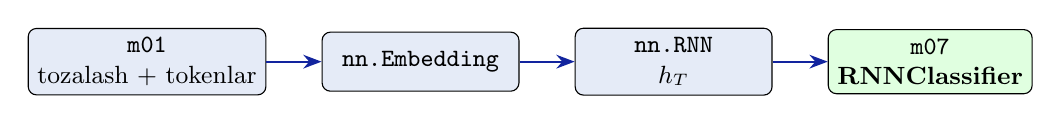
\begin{tikzpicture}[
      mod/.style={draw, fill=cnubluebg, rounded corners=3pt,
                  minimum width=2.5cm, minimum height=0.75cm,
                  font=\small, align=center},
      fin/.style={draw, fill=green!12, rounded corners=3pt,
                  minimum width=2.5cm, minimum height=0.75cm,
                  font=\small\bfseries, align=center},
      arr/.style={-{Stealth}, thick, color=cnublue}
  ]
    \node[mod] (cl) {\texttt{m01}\\ tozalash + tokenlar};
    \node[mod, right=0.7cm of cl]  (em) {\texttt{nn.Embedding}};
    \node[mod, right=0.7cm of em]  (rn) {\texttt{nn.RNN}\\ $h_T$};
    \node[fin, right=0.7cm of rn]  (m7) {\texttt{m07}\\ RNNClassifier};
    \draw[arr] (cl)--(em); \draw[arr] (em)--(rn); \draw[arr] (rn)--(m7);
  \end{tikzpicture}
  \end{center}
  \vspace{5pt}
  \begin{columns}[T]
    \begin{column}{0.50\textwidth}
      \textbf{P7 da qurasiz:}\\[3pt]
      \small
      \begin{itemize}\setlength\itemsep{2pt}
        \item \texttt{m07 RNNClassifier}: Embedding $+$ \texttt{nn.RNN} $+$ Linear
        \item \texttt{ijobiy}/\texttt{salbiy} tasniflash, F1 baho
        \item RNN bir qadami $h_1$ ni tekshirish
      \end{itemize}
    \end{column}
    \begin{column}{0.46\textwidth}
      \textbf{Birinchi assert (bu slayd [I2]):}\\[4pt]
      \small\ttfamily
      assert np.allclose(\\
      \phantom{xx}h1, [0.762, 0.0],\\
      \phantom{xx}atol=1e-3)\\[4pt]
      \normalfont\footnotesize\color{halfgray}
      \textit{\# Ma'ruza L7 [I2]-slayd bilan}\\
      \textit{\# solishtiring (RNN bir qadami)}
    \end{column}
  \end{columns}
\end{frame}

% ----------------------------------------------------------------
% [R] ADABIYOTLAR
% ----------------------------------------------------------------
\begin{frame}{Adabiyotlar}
  \begin{enumerate}\small\setlength\itemsep{5pt}
    \item Rumelhart, D.E., Hinton, G.E., Williams, R.J.\ (1986). \textit{Learning
          Representations by Back-Propagating Errors.} Nature 323:533--536.
    \item Elman, J.L.\ (1990). \textit{Finding Structure in Time.} Cognitive
          Science 14(2). (Oddiy rekurrent tarmoq.)
    \item Werbos, P.J.\ (1990). \textit{Backpropagation Through Time.} Proc. IEEE 78(10).
    \item Jurafsky, D., Martin, J.H.\ (2023). \textit{Speech and Language
          Processing}, 3-nashr. 9-bob: RNN va LSTM.
    \item \texttt{torch.nn.RNN} hujjatlari --- PyTorch rekurrent qatlamlar.
  \end{enumerate}
\end{frame}

% ================================================================
% [S] ILOVALAR (appendix --- slayd soniga kirmaydi)
% ================================================================
\appendix

\begin{frame}{Ilova S1: BPTT --- gradientlarning yig'ilishi}
  \small
  $W_h$ barcha qadamlarda ulashilgani uchun to'liq gradient har qadam hissasining
  yig'indisi:
  $$ \frac{\partial \mathcal{L}}{\partial W_h}
     = \sum_{t=1}^{T}\ \sum_{s=1}^{t}
       \frac{\partial \mathcal{L}_t}{\partial h_t}
       \Big(\prod_{r=s+1}^{t}\frac{\partial h_r}{\partial h_{r-1}}\Big)
       \frac{\partial h_s}{\partial W_h} $$
  \bunda{ichki ko'paytma --- $s$ dan $t$ gacha bo'lgan zanjir; aynan shu ko'paytma
  uzoq masofada so'nadi yoki portlaydi.}
  \vspace{4pt}

  Amalda: gradient kesish (clipping) portlashni, LSTM/GRU darvozalari so'nishni
  yumshatadi.
\end{frame}

\begin{frame}{Ilova S2: nega aynan $\tanh$?}
  \small
  $\tanh$ chiqishni $[-1,1]$ ga siqadi --- holat qiymatlari portlamaydi va
  markazlashgan (0 atrofida), bu o'qitishni barqarorlashtiradi.
  $$ \tanh'(x) = 1 - \tanh^2(x) \in (0,\,1] $$
  \bunda{hosila $\leq 1$ bo'lgani uchun ko'p qadam ko'paytmasi so'nishga moyil ---
  vanishing gradientning matematik ildizi.}
  \vspace{4pt}

  Muqobil: ReLU tez, ammo rekurrentda beqaror bo'lishi mumkin; shuning uchun klassik
  RNN $\tanh$ ishlatadi.
\end{frame}

\end{document}
